\documentclass{article}

% if you need to pass options to natbib, use, e.g.:
%     \PassOptionsToPackage{numbers, compress}{natbib}
% before loading neurips_2025

% The authors should use one of these tracks.
% Before accepting by the NeurIPS conference, select one of the options below.
% 0. "default" for submission
\usepackage{amsmath}
\usepackage{graphicx}
\usepackage[sglblindworkshop]{neurips_2025}
% the "default" option is equal to the "main" option, which is used for the Main Track with double-blind reviewing.
% 1. "main" option is used for the Main Track
%  \usepackage[main]{neurips_2025}
% 2. "position" option is used for the Position Paper Track
%  \usepackage[position]{neurips_2025}
% 3. "dandb" option is used for the Datasets & Benchmarks Track
 % \usepackage[dandb]{neurips_2025}
% 4. "creativeai" option is used for the Creative AI Track
%  \usepackage[creativeai]{neurips_2025}
% 5. "sglblindworkshop" option is used for the Workshop with single-blind reviewing
 % \usepackage[sglblindworkshop]{neurips_2025}
% 6. "dblblindworkshop" option is used for the Workshop with double-blind reviewing
%  \usepackage[dblblindworkshop]{neurips_2025}

% After being accepted, the authors should add "final" behind the track to compile a camera-ready version.
% 1. Main Track
 % \usepackage[main, final]{neurips_2025}
% 2. Position Paper Track
%  \usepackage[position, final]{neurips_2025}
% 3. Datasets & Benchmarks Track
 % \usepackage[dandb, final]{neurips_2025}
% 4. Creative AI Track
%  \usepackage[creativeai, final]{neurips_2025}
% 5. Workshop with single-blind reviewing
%  \usepackage[sglblindworkshop, final]{neurips_2025}
% 6. Workshop with double-blind reviewing
%  \usepackage[dblblindworkshop, final]{neurips_2025}
% Note. For the workshop paper template, both \title{} and \workshoptitle{} are required, with the former indicating the paper title shown in the title and the latter indicating the workshop title displayed in the footnote.
% For workshops (5., 6.), the authors should add the name of the workshop, "\workshoptitle" command is used to set the workshop title.
% \workshoptitle{WORKSHOP TITLE}

% "preprint" option is used for arXiv or other preprint submissions
 % \usepackage[preprint]{neurips_2025}

% to avoid loading the natbib package, add option nonatbib:
%    \usepackage[nonatbib]{neurips_2025}

\usepackage[utf8]{inputenc} % allow utf-8 input
\usepackage[T1]{fontenc}    % use 8-bit T1 fonts
\usepackage{hyperref}       % hyperlinks
\usepackage{url}            % simple URL typesetting
\usepackage{booktabs}       % professional-quality tables
\usepackage{amsfonts}       % blackboard math symbols
\usepackage{nicefrac}       % compact symbols for 1/2, etc.
\usepackage{microtype}      % microtypography
\usepackage{xcolor}         % colors

% Note. For the workshop paper template, both \title{} and \workshoptitle{} are required, with the former indicating the paper title shown in the title and the latter indicating the workshop title displayed in the footnote. 
\title{Emergent Reasoning Networks for Multi-Agent Knowledge Graph Validation}

\workshoptitle{NORA: The First Workshop on Knowledge Graphs \& Agentic Systems Interplay}
% The \author macro works with any number of authors. There are two commands
% used to separate the names and addresses of multiple authors: \And and \AND.
%
% Using \And between authors leaves it to LaTeX to determine where to break the
% lines. Using \AND forces a line break at that point. So, if LaTeX puts 3 of 4
% authors names on the first line, and the last on the second line, try using
% \AND instead of \And before the third author name.


\author{%
  Pragya Singh\thanks{Equal Contribution}\\
  University of Pennsylvania\\
  \texttt{pragya7@seas.upenn.edu} \\
  % examples of more authors
  \And
  Stanley Yu\footnotemark[1]\\
  University of Pennsylvania \\
  \texttt{stany@seas.upenn.edu} \\
  % \AND
  % Coauthor \\
  % Affiliation \\
  % Address \\
  % \texttt{email} \\
  % \And
  % Coauthor \\
  % Affiliation \\
  % Address \\
  % \texttt{email} \\
  % \And
  % Coauthor \\
  % Affiliation \\
  % Address \\
  % \texttt{email} \\
}


\begin{document}


\maketitle


\begin{abstract}
  LLM-based agents struggle with persistent challenges of catastrophic forgetting, context limitations, and reasoning drift. While knowledge graphs (KGs) offer structured memory, current implementations remain static and do not adapt based on reasoning effectiveness. We introduce Kairos, a multi-agent reasoning system featuring an adaptive KG that evolves via Hebbian plasticity. This approach allows the graph to learn from experience: frequently-validated reasoning paths are strengthened, while unused connections decay. A key innovation is our validation-gated mechanism. To prevent the reinforcement of hallucinations, only reasoning paths passing a multi-dimensional quality assessment trigger consolidation. Kairos serves as an initial exploration into systems using KGs as adaptive cognitive structures that learn from validated experience, aiming to create more robust and reliable agent reasoning.
\end{abstract}

\section{Introduction}

Large language model (LLM)-based agents face persistent challenges with long-term memory and reasoning stability, hindered by catastrophic forgetting~\citep{li-etal-2024-revisiting,luo2023empirical}, context window limitations~\citep{packer2023memgpt}, and reasoning drift~\citep{chen2023chatgpt}. The degradation can be stark: one study showed GPT-4's accuracy on a simple task falling dramatically in just three months~\citep{chen2023chatgpt}. Expanded context windows are not a panacea, introducing quadratic costs and the "lost in the middle" effect where information is ignored~\citep{packer2023memgpt}.

Knowledge graphs (KGs) have emerged as a promising architecture to address this, providing structured representations for complex, multi-hop reasoning~\citep{pan2024unifying}. Systems like GraphRAG, MemGPT, and A-Mem confirm that structured knowledge provides a more robust foundation for agent memory than raw context accumulation, improving retrieval and multi-hop reasoning~\citep{edge2024graphrag,packer2023memgpt,xu2025amem}.

A critical gap remains: current KG-based systems treat the graph as a static database. While graphs may grow through data ingestion~\citep{edge2024graphrag} or agents may adapt navigation strategies~\citep{chen2024pog}, the graph's underlying structure rarely learns from the agent's reasoning. Connections are not strengthened by successful use, and ineffective pathways do not weaken, representing a missed opportunity for adaptive knowledge consolidation.

This gap provides an opportunity to draw from biological memory, where synaptic connections strengthen through repeated co-activation—the Hebbian principle of "neurons that fire together wire together"~\citep{hebb1949organization,squire2015memory}. This inspires a model where a KG evolves based on its utility. While some work explores generative graph expansion~\citep{buehler2025agentic}, our work focuses on optimizing the graph structure through validation-based learning.

We present Kairos, a multi-agent reasoning system that explores Hebbian plasticity mechanisms for knowledge graphs. Kairos treats KGs as adaptive cognitive structures that evolve based on reasoning outcomes. Successful reasoning paths are strengthened (long-term potentiation), unused edges weaken (long-term depression), and frequently co-activated concepts form emergent connections. Critically, this adaptation is **validation-gated**: only reasoning paths passing multi-dimensional quality assessment (e.g., logical consistency, factual grounding) trigger consolidation. This mechanism is designed to prevent the reinforcement of hallucinations.

Our key contributions are:
\begin{itemize}
    \item \textbf{Hebbian plasticity mechanisms for knowledge graphs}: Implementation of adaptive edge strengthening (LTP analog), temporal decay (LTD analog), and emergent connection formation based on agent co-activation patterns.
    \item \textbf{Validation-gated learning framework}: A multi-agent validation architecture (logical, grounding, novelty, and alignment) that gates knowledge consolidation, ensuring graph structure strengthens based on quality, not just frequency.
    \item \textbf{Episodic-to-semantic memory transition}: A concrete implementation where reasoning episodes (query-answer pairs) gradually strengthen semantic knowledge (graph structure), inspired by biological memory.
    \item \textbf{End-to-end demonstration system}: A functional implementation spanning document ingestion, specialized reasoning modules, validation, and adaptive graph evolution.
\end{itemize}

Kairos contributes to the synergy between LLM agents and KGs by exploring how graphs can serve as adaptive agent memory that learns from validated experience.

\section{Related Work}

\subsection{Graph-Based Retrieval and Reasoning Systems}

Graph RAG systems improve retrieval, but their underlying structures are often static. Microsoft's GraphRAG pre-generates hierarchical summaries that do not adapt to queries~\citep{edge2024graphrag}. Similarly, reasoning-over-graphs~\citep{luo2024rog} and hybrid vector-KG systems~\citep{sarmah2024hybridrag} typically operate on fixed graphs. Even systems with adaptive planning, like Plan-on-Graph, refine exploration strategies over a static graph structure~\citep{chen2024pog}.

\subsection{Agent Memory Architectures}

Agent memory systems have evolved, but often rely on static retrieval mechanisms. MemGPT pioneered hierarchical memory~\citep{packer2023memgpt}, and A-Mem implements linkable atomic notes~\citep{xu2025amem}. While A-Mem's notes "evolve," the retrieval mechanism itself remains a static top-k similarity search. Other multi-agent systems use KGs for construction~\citep{liang2023cooperkgc} or structural organization~\citep{zhang2024graphs}, not as an adaptive reasoning memory.

\subsection{Dynamic Knowledge Graphs and Continual Learning}

Existing dynamic KGs typically adapt to *new data*, not reasoning quality. Know-Evolve updates embeddings based on event streams~\citep{trivedi2017knowevolve}, and LLM-DA adapts temporal rules as new events occur~\citep{wang2024llmda}. Other work demonstrates generative graph expansion during reasoning~\citep{buehler2025agentic}. Continual learning approaches focus on accommodating new entities into a graph without catastrophic forgetting~\citep{daruna2021continual}, rather than optimizing existing connections based on use.

\subsection{Neuroscience-Inspired Learning Mechanisms}

Hebbian principles have been applied to GNNs for tasks like multi-view data fusion~\citep{mvil2024hebbian}, but their application to symbolic agent reasoning is exploratory. This aligns with the "dynamic rule learning" challenge identified in neural-symbolic AI research~\citep{yang2025neuralsymbolic}, where integrating learning-based evolution with symbolic structures remains an active challenge.

\subsection{Positioning Kairos}

Kairos integrates three threads: (1) the retrieval effectiveness of graph RAG systems~\citep{edge2024graphrag}, (2) the sophisticated memory management of architectures like MemGPT and A-Mem~\citep{packer2023memgpt,xu2025amem}, and (3) the principles of Hebbian plasticity~\citep{hebb1949organization}. While existing systems excel at organizing knowledge (GraphRAG), managing memory access (MemGPT), or evolving via data arrival (Know-Evolve), Kairos explores a different dimension: \textit{learning which knowledge structures support successful reasoning}. By applying validation-gated plasticity, Kairos investigates whether KGs can become adaptive cognitive substrates that improve through validated use, moving beyond static organizational or retrieval-focused roles.

\section{System Architecture}

Kairos implements a pipeline that integrates document ingestion, multi-agent reasoning, validation, and adaptive knowledge consolidation. Figure~\ref{fig:architecture} illustrates the system's core components and information flow.

\begin{figure}
    \centering
    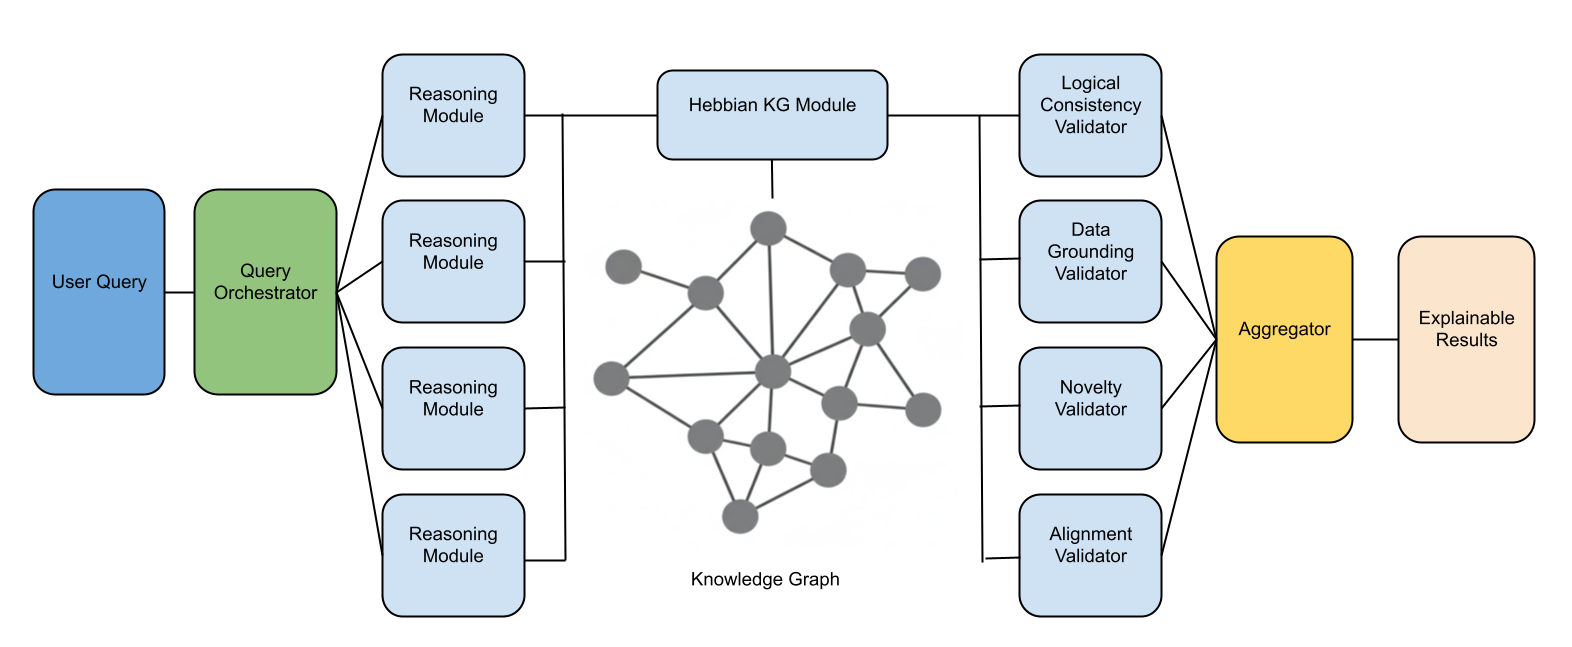
\includegraphics[width=\linewidth]{fig/Kairos (1).png}
    \caption{The Kairos system architecture. A user query is processed by an orchestrator, specialized reasoning modules, and a multi-agent validation layer. These components interact with a central knowledge graph, which is dynamically updated by a Hebbian KG module.}
    \label{fig:architecture}
\end{figure}

\subsection{Core Components}

\textbf{Query Orchestrator.} The orchestrator serves as the system's entry point, receiving user queries and routing them to appropriate reasoning modules. Module selection employs semantic similarity computed via sentence transformers (all-MiniLM-L6-v2)~\citep{reimers2019sentencebert}, matching query embeddings against module descriptions. For complex queries requiring multiple perspectives, the orchestrator can invoke several modules sequentially or in parallel.

\textbf{Specialized Reasoning Modules.} Kairos can be configured with any number of specialized reasoning modules. For our demonstration, we implement four such modules, each a specialized LLM fine-tuned for a distinct reasoning function (e.g., data synthesis, trend analysis, causal inference). This four-module setup is one example tailored for a specific complex analysis use case, but the architecture is flexible.

Each module queries the knowledge graph to retrieve relevant entities and relationships, constructs a reasoning path explaining its inference process, and produces a structured output containing: (1) a step-by-step reasoning path with data sources and logical inferences, (2) a conclusion with confidence score, (3) the specific KG triples used (source\_triples), and (4) relevant metrics. This structured output enables downstream validation and Hebbian learning by making explicit which graph elements contributed to the reasoning.

\textbf{Dynamic Knowledge Graph.} The knowledge graph represents information as entity-relation triples with rich metadata. Each relation stores not only subject-predicate-object structure but also a confidence score (0.0-1.0), source provenance, temporal versioning, and Hebbian-specific metadata including activation count and last-used timestamp. This metadata enables the system to track usage patterns over time. The graph supports both static triples extracted during document ingestion and emergent relations formed through co-activation patterns during reasoning.

\textbf{Multi-Agent Validation Layer.} Four specialized validation agents assess reasoning quality from complementary perspectives before any graph adaptation occurs. This diversity of validation helps prevent premature consolidation of flawed reasoning patterns~\citep{xu2025amem}. The validation layer outputs numerical scores (0-1) and textual feedback for each dimension, which gate the Hebbian learning process.

\subsection{Validation-Gated Learning Feedback Loop}

The critical architectural feature distinguishing Kairos from prior work is the validation gate between reasoning and learning. When a reasoning module produces output, validation agents assess quality across four dimensions (detailed in Section~\ref{sec:validation}). Only when \textit{all} validators indicate acceptable quality (scores above threshold) does the system trigger Hebbian updates to strengthen the edges traversed during reasoning. This gate serves two purposes: (1) it prevents consolidation of hallucinated facts or logically incoherent reasoning paths, and (2) it aligns with neuroscientific findings that successful task completion, not mere neural activity, drives synaptic strengthening~\citep{squire2015memory}.

Failed reasoning attempts—those producing low validation scores—do not trigger edge strengthening, though temporal decay continues to operate on unused edges independently. This asymmetric update policy mirrors biological learning, where successful behaviors are reinforced while unsuccessful attempts gradually fade from memory without explicit negative reinforcement.

\section{Hebbian Plasticity for Knowledge Graphs}
\label{sec:hebbian}

\subsection{Motivation: Beyond Static Knowledge Organization}

Current agent knowledge graphs (KGs) are often static, requiring agents to re-explore paths with equal effort even as reasoning patterns evolve. An adaptive graph, by contrast, would learn to make frequently successful reasoning paths more accessible, reducing latency and improving response quality~\citep{packer2023memgpt}.

We draw inspiration from biological memory, where synaptic plasticity—long-term potentiation (LTP) and long-term depression (LTD)—strengthens or weakens neural connections based on use~\citep{hebb1949organization,squire2015memory}. While these principles have been applied to ANNs~\citep{mvil2024hebbian}, their application to symbolic KG structures in agentic systems remains exploratory.

Kairos investigates these mechanisms for KG-based agent memory. Our hypothesis is that edges traversed during \textit{validated} reasoning should strengthen, unused edges should weaken, and frequently co-activated entities should form emergent connections.

\subsection{Mechanisms}

\subsubsection{Edge Strengthening: Long-Term Potentiation Analog}

When a reasoning module's output passes validation, the KG edges listed in its \texttt{source\_triples} field receive a strengthening signal. We implement asymptotic strengthening with diminishing returns:

\begin{equation}
\Delta_{\text{strength}} = \eta \times (\text{max\_strength} - \text{current\_strength})
\label{eq:ltp}
\end{equation}

\begin{equation}
\text{new\_strength} = \min(\text{max\_strength}, \text{current\_strength} + \Delta_{\text{strength}})
\end{equation}

where $\eta = 0.1$ is the learning rate and $\text{max\_strength} = 1.0$. This formulation mirrors biological LTP~\citep{squire2015memory}, allowing for noticeable adaptation within 10-20 episodes while preventing single-trial over-consolidation. For multi-hop paths, each edge receives proportional strengthening.

\subsubsection{Temporal Decay: Long-Term Depression Analog}

Edges not traversed during reasoning gradually weaken via temporal decay, analogous to synaptic depression~\citep{squire2015memory}. We implement exponential decay with a 30-day half-life:

\begin{equation}
\text{decay} = \gamma \times \left(1 - \exp\left(-\frac{\text{days\_inactive}}{30}\right)\right)
\label{eq:ltd}
\end{equation}

\begin{equation}
\text{new\_strength} = \max(\text{min\_strength}, \text{current\_strength} - \text{decay})
\end{equation}

where $\gamma = 0.05$ is the decay rate and $\text{min\_strength} = 0.1$ is a pruning threshold. This mechanism balances knowledge retention against the removal of irrelevant associations, allowing the graph to adapt to changing usage patterns while preventing catastrophic forgetting.

\subsubsection{Emergent Connection Formation}

Kairos also forms emergent relationships by tracking entity co-activations. When two entities appear in the same validated \texttt{source\_triples} $N=3$ times, a new \texttt{co\_occurs\_with} edge is created:

\begin{equation}
\text{initial\_strength} = \min\left(0.5, \frac{\text{co\_activation\_count}}{N + 2}\right)
\end{equation}

This discovers implicit, cross-domain connections. The threshold $N=3$ reduces noise, and the initial strength is capped at 0.5 to distinguish empirical edges from source-derived facts.

\textbf{Example:} If entities \texttt{Security-Audit} and \texttt{High-Risk} are co-activated three times across different security analysis queries, Kairos creates an emergent edge:

\begin{center}
\texttt{Security-Audit --[co\_occurs\_with, strength=0.3]--> High-Risk}
\end{center}

This new connection captures an empirical pattern (audits co-occur with high-risk findings) that can accelerate future reasoning.

\begin{equation}
\text{trigger\_hebbian} \leftarrow \begin{cases}
\text{True} & \text{if all } v_i > \theta_i \\
\text{False} & \text{otherwise}
\end{cases}
\end{equation}

where $v_i$ are validation scores and $\theta_i$ are per-validator thresholds (e.g., 0.7 for grounding, 0.5 for novelty). This implements a form of quality-aware reinforcement, inspired by reward signals in biological learning~\citep{squire2015memory}, to prevent the consolidation of poor reasoning.

\section{Multi-Dimensional Validation Framework}
\label{sec:validation}

Kairos employs four specialized validation agents that assess reasoning quality from complementary perspectives, acknowledging that single-dimensional evaluation is insufficient for complex reasoning~\citep{park2023generative,xu2025amem}.

\subsection{Logical Validation (LogicalVN)}

Analyzes the coherence of reasoning paths using an LLM (GPT-4) to check for contradictions and logical fallacies (e.g., circular reasoning). It outputs a 0-1 score and textual feedback. While LLM-based logical assessment has limitations, it provides a practical proxy for coherence~\citep{pan2024unifying}.

\subsection{Grounding Validation (GroundingVN)}

Verifies that reasoning claims are anchored in KG facts. The validator parses claimed triples from the reasoning path, queries the KG, and computes a grounding ratio:

\begin{equation}
\text{grounding\_score} = \frac{\text{verified\_triples}}{\text{total\_claimed\_triples}}
\end{equation}

A 1.0 score indicates all claims are grounded. This is critical for preventing the consolidation of logically coherent but factually incorrect hallucinations~\citep{edge2024graphrag}.

\subsection{Novelty Validation (NoveltyVN)}

Assesses whether a conclusion is an emergent insight or a restatement of existing knowledge by comparing it to KG entities via semantic similarity. This validator's purpose is not to gate poor reasoning, but to identify novel synthesis. Thus, its threshold (e.g., 0.5) is typically lower than quality-focused validators (e.g., 0.7).

\subsection{Alignment Validation (AlignmentVN)}

Checks whether reasoning respects user-defined preferences, goals, and ethical constraints (e.g., "prioritize risk mitigation"). It uses an LLM to assess reasoning against these constraints. While comprehensive alignment specification remains an open challenge~\citep{pan2024unifying}, this module provides a necessary architectural provision for safe deployment.

\subsection{Trust Score Aggregation}

After all four validators produce scores, Kairos computes an aggregate trust score via simple averaging:

\begin{equation}
\text{trust\_score} = \frac{1}{4} \sum_{i=1}^{4} v_i
\end{equation}

where $v_i \in [0,1]$ are the four validation scores. This simple aggregation treats all dimensions as equally important. More sophisticated aggregation schemes (e.g., weighted averages, minimum-operator) could be explored in future work.
\section{Results}

ermm

\section{Discussion and Future Work}
\label{sec:discussion}

\subsection{Discussion}

Kairos explores the application of Hebbian plasticity principles to knowledge graphs in multi-agent reasoning systems. The key insight is that knowledge graphs need not remain static organizational structures but can evolve based on validated reasoning patterns, potentially learning which connections support successful task completion. By gating adaptation on multi-dimensional validation, the system aims to reinforce high-quality reasoning paths while preventing consolidation of hallucinations or flawed logic.

This work suggests several implications for agent memory architectures. First, the distinction between episodic memory (individual reasoning episodes) and semantic memory (graph structure) can be bridged through consolidation mechanisms that gradually strengthen frequently-validated patterns~\citep{squire2015memory}. Second, neuroscience-inspired learning mechanisms like Hebbian plasticity can be formalized for symbolic structures, not just neural networks~\citep{mvil2024hebbian}. Third, validation-gated learning provides a potential approach for quality-aware knowledge consolidation, though the effectiveness of this approach requires empirical evaluation on benchmark tasks.

\subsection{Limitations}

Several limitations warrant acknowledgment. \textbf{Scale:} The current JSON-based knowledge graph implementation handles graphs with thousands of nodes but would face performance challenges with millions of entities. Migration to dedicated graph databases (Neo4j, Neptune) would be necessary for large-scale deployment~\citep{edge2024graphrag}. \textbf{Evaluation:} We provide qualitative demonstrations but lack quantitative evaluation against established benchmarks. Rigorous assessment would require metrics that measure graph quality evolution over time, such as query response accuracy across episodes, reasoning efficiency (path length/latency), and knowledge transfer to novel but related tasks. \textbf{Hyperparameters:} Learning rate ($\eta = 0.1$), decay rate ($\gamma = 0.05$), and co-activation threshold ($N = 3$) were chosen through informal experimentation rather than systematic optimization. Different task domains may require different parameter settings.

\textbf{Validation reliability:} The current validation layer relies heavily on LLM-based assessment, which inherits limitations of the underlying models including potential biases, inconsistent evaluation across queries, and difficulty with complex logical reasoning~\citep{pan2024unifying}. More robust validation might incorporate formal verification tools for logical validation, deterministic fact-checking for grounding, and explicit user feedback for alignment. \textbf{Causality:} The system strengthens edges based on correlation with successful reasoning but cannot distinguish causal contributions from coincidental co-occurrence. An edge might strengthen simply because it appears in reasoning paths that succeed for other reasons.

\subsection{Future Directions}

Several extensions could improve Kairos's capabilities. \textbf{Graph Neural Networks:} Integrating GNN-based reasoning over graph structure could enable more sophisticated pattern recognition and multi-hop inference beyond simple path traversal~\citep{luo2024rog}. \textbf{Adaptive module selection:} Learning optimal module routing from feedback, rather than relying solely on semantic similarity, could improve orchestration~\citep{chen2024pog}. \textbf{Continuous learning from user feedback:} Incorporating explicit user corrections or ratings could provide stronger signals for validation than automated validators alone~\citep{xu2025amem}.

\textbf{Multi-modal knowledge integration:} Extending the knowledge graph to support images, tables, and code as first-class entities would enable richer reasoning in domains like technical documentation analysis or scientific literature review~\citep{edge2024graphrag}. \textbf{Distributed validation:} Scaling validation across multiple nodes could reduce latency for high-throughput applications. \textbf{Explanation generation:} Producing natural language explanations of reasoning paths and Hebbian updates would improve interpretability and enable users to understand why the system strengthened or weakened specific connections.

\textbf{Comparative evaluation:} Systematic comparison against static graph baselines (GraphRAG, MemGPT, A-Mem) on standardized benchmarks would quantify the benefits of adaptive consolidation. Key metrics might include: accuracy improvement over episodes, knowledge transfer to novel queries, resilience to distribution shift, and computational efficiency (amortized cost per query as graph adapts). Such evaluation would help determine whether adaptive knowledge consolidation provides meaningful advantages over simpler static approaches in practice.

\section{Conclusion}

We presented Kairos, a multi-agent reasoning system that explores Hebbian plasticity mechanisms for knowledge graphs with validation-driven adaptation. By implementing edge strengthening analogous to long-term potentiation, temporal decay analogous to long-term depression, and emergent connection formation based on co-activation patterns, Kairos investigates whether knowledge graphs can learn from reasoning experience rather than remaining static organizational structures. The critical design choice of validation-gated learning—where only high-quality reasoning triggers consolidation—aims to prevent reinforcement of hallucinations while allowing useful patterns to strengthen.

\bibliographystyle{plainnat}
\bibliography{references}

\appendix

\section{Implementation Details}
\label{appendix:implementation}

\subsection{Technical Stack}

\textbf{Backend:}
\begin{itemize}
\item Language: Python 3.8+
\item Web Framework: FastAPI 0.104.0, Flask 3.0.0
\item LLM API: OpenAI GPT-4 (gpt-4-0613)
\item Embeddings: Sentence Transformers 2.2.0 (all-MiniLM-L6-v2 model)
\item NLP: spaCy 3.7.0, Transformers 4.35.0
\item Knowledge Graph Storage: JSON-based with in-memory processing
\item OCR: Upstage Document Parse API
\end{itemize}

\textbf{Frontend:}
\begin{itemize}
\item Framework: Next.js 14.0.0, React 18.2.0
\item UI Components: Radix UI, Tailwind CSS 3.3.0
\item Language: TypeScript 5.2.0
\end{itemize}

\subsection{Computational Resources}

Development and demonstration runs were conducted on standard CPU infrastructure without specialized hardware acceleration. The system does not require GPU resources for core functionality, as reasoning and validation leverage cloud-based LLM APIs (Anthropic Claude-3 Haiku). Sentence transformer embeddings (all-MiniLM-L6-v2) run efficiently on CPU for the scales demonstrated (knowledge graphs with 1000-5000 entities).

For production deployment at larger scales, GPU acceleration would benefit embedding computation and enable local LLM inference, though the current cloud API approach was chosen for accessibility and reproducibility.

\subsection{Hyperparameters}

Key hyperparameters for Hebbian learning mechanisms:
\begin{itemize}
\item Learning rate ($\eta$): 0.1
\item Maximum edge strength: 1.0
\item Decay rate ($\gamma$): 0.05
\item Temporal decay half-life: 30 days
\item Minimum edge strength (pruning threshold): 0.1
\item Co-activation threshold ($N$): 3
\item Validation pass thresholds: 0.7 (logical, grounding), 0.5 (novelty, alignment)
\end{itemize}

\subsection{Code Availability}

Complete source code, documentation, usage examples, and demonstration scenarios are available in the project repository: \url{https://github.com/pragya-s7/Emergent-Reasoning-Networks}.
\end{document}

